
\pgfplotsset{every axis plot/.append style={line width=2pt}}
\tikzset{
every pin/.style={fill=yellow!50!white,rectangle,rounded corners=3pt,font=\tiny},
small dot/.style={fill=black,circle,scale=0.3}
}
\begin{figure}
\centering
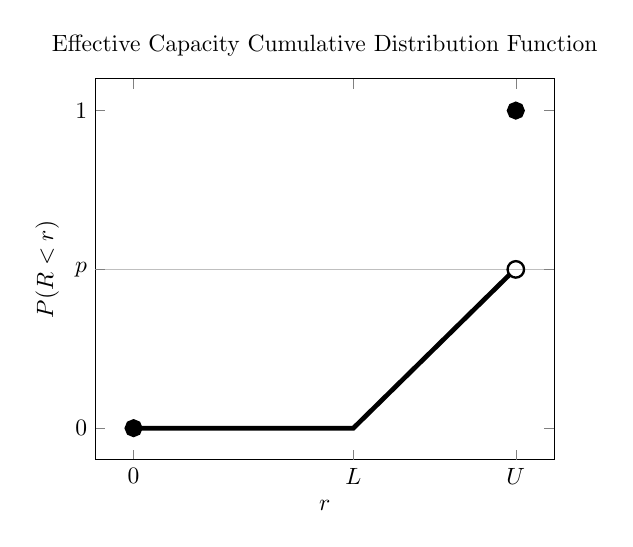
\begin{tikzpicture}[scale=.85]
\begin{axis}[ 
	xlabel=$r$,
	ylabel=$P( R < r )$,
	title = Effective Capacity Cumulative Distribution Function,
	unbounded coords = jump,
	xtick= {0},
	ytick= {0, 1},
	extra y ticks={.5},
	extra y tick style={grid=major},
	extra y tick labels={$p$},
	extra x ticks={.575,1},
	extra x tick labels={$L$, $U$},
scatter/classes={
 		 a={mark=o,line width=3.5pt},%
 		 b={mark=o,line width=1pt,scale=1.75}%
		}]
	\addplot[black] coordinates { 
		(0,0)		
		(.575,0)	
		(.985,.485) 		
		(1,inf)		
		(1,1)		
		};	
	\addplot[ 
		scatter,only marks,
		scatter src=explicit symbolic]
		coordinates {  
		(0,0)		[a]
		(1,.5)		[b]
		(1,1)		[a]
		};


	

\end{axis}
\end{tikzpicture}

\caption{ Example Effective Capacity Distribution for equation (\ref{r}) }
\label{cdf}
\end{figure}
